%%%% main.tex -- Depth-Aware Polka Dot Art Generation (IJCAI'26 Arts track)
% Based on the official IJCAI--ECAI 26 template (ijcai26.sty).

\typeout{IJCAI--ECAI 26 Submission: Depth-Aware Polka Dot Art Generation}

\documentclass{article}
\pdfpagewidth=8.5in
\pdfpageheight=11in

\usepackage{ijcai26}

\usepackage{times}
\usepackage{soul}
\usepackage{url}
\usepackage[hidelinks]{hyperref}
\usepackage[small]{caption}
\usepackage{graphicx}
\usepackage{amsmath}
\usepackage{amssymb}
\usepackage{amsthm}
\usepackage{natbib}
\usepackage{booktabs}
\usepackage{algorithm}
\usepackage{algorithmic}
\usepackage[switch]{lineno}
\usepackage{xcolor}
\usepackage{tikz}
\usetikzlibrary{arrows.meta,positioning,calc}

\linenumbers

\urlstyle{same}

\newtheorem{definition}{Definition}
\newtheorem{proposition}{Proposition}

\ifdefined\pdfinfo
\pdfinfo{
/TemplateVersion (IJCAI.2026.0)
}
\fi

% =====================================================================
%  Title and authors
% =====================================================================
\title{Depth-as-Radius: Kusama-Style Polka Dot Generation\\
via Monocular Vision and Three-Layer Voronoi Stippling}

\author{
    Anonymous Authors
    \affiliations
    AIforEducation Project
    \emails
    aiforeducation@example.com
}

\begin{document}

\maketitle

\begin{abstract}
We present \emph{Depth-as-Radius}, a non-photorealistic rendering
pipeline that translates a single RGB image into a Yayoi
Kusama--style polka dot composition in which dot size---rather
than luminance---encodes scene depth. The key idea is a simple
yet expressive depth-to-radius mapping: a per-pixel monocular
depth estimate is normalized over the foreground region and
passed through a power-law falloff with multiplicative Gaussian
jitter, so that near surfaces receive large, prominent dots
while distant content dissolves into fields of fine specks.
Combined with a semantic segmentation mask, the same pipeline
assigns distinct dot colors to foreground and background,
producing a figure--ground separation that echoes Kusama's
installation practice.

Algorithmically, the pipeline couples a modern unified vision
backbone (YOLO26, used for both depth estimation and semantic
segmentation) with a three-layer Weighted Voronoi stippling
architecture. A fine-stipple layer provides dense texture; a
depth-emphasis layer places large dots only in near regions;
an edge-and-background layer completes the horror-vacui
coverage. A dedicated cross-layer overlap-pruning step
guarantees that large dots remain visually distinct from the
fine texture, which is essential at the extreme radius range
(roughly 1--15\,px) that our depth mapping demands.

Experiments on three natural images and five Kusama palettes
show that the method produces controllable depth encoding
(radius span 0.5--15.4\,px within a single composition),
preserves dot separation (maximum blob ratio below 0.65\%
of canvas), and supports intuitive artistic control through
a small set of interpretable parameters. Our results suggest
that pretrained monocular vision models---originally trained
for autonomous driving---can serve as practical artistic
primitives, supplying geometric and semantic control signals
that purely luminance-based stippling cannot express.
\end{abstract}

% =====================================================================
%  Body
% =====================================================================
\section{Introduction}
\label{sec:introduction}

Yayoi Kusama (born 1929) is one of the most influential living artists,
renowned for her obsessive deployment of polka dots across paintings,
sculptures, and immersive installations. Her visual language is built
upon four signature traits: geometrically precise hard-edged dots,
multi-scale coexistence of dot sizes ranging from sub-millimeter specks
to large medallions, ultra-pure high-chroma color palettes applied in
flat fields, and \emph{horror vacui}---a compulsion to cover every
available surface with dots, leaving no void untouched
\citep{moma_kusama,archdaily_kusama}. The polka dot, in
Kusama's universe, is simultaneously a decorative motif, a signifier of
infinity, and a mechanism for dissolving the boundary between the self
and the environment.

Translating this artistic language into a computational framework
presents a unique set of challenges. Classical stippling algorithms,
pioneered by \citet{secord2002weighted} and grounded in Centroidal
Voronoi Tessellation (CVT) and Lloyd relaxation \citep{lloyd1982least},
excel at producing blue-noise point distributions modulated by image
density. However, these methods map dot size and density to a single
scalar field---typically luminance: dark regions receive larger or
denser dots, bright regions receive fewer and smaller ones. This
one-dimensional mapping is fundamentally at odds with Kusama's
practice. A pumpkin painted by Kusama does not merely have dots of
varying size due to shading; the dots themselves carry a sense of
volume, of near and far, of the object inhabiting space. Capturing
this requires a control signal that luminance alone cannot provide.

Monocular depth estimation supplies exactly such a signal. The field
has matured rapidly, and recent unified real-time backbones---most
notably the YOLO26 family \citep{ultralytics2025yolo26}---now produce
dense metric depth maps at interactive rates on consumer GPUs. Three
considerations motivate our choice of YOLO26 over alternatives such as
MiDaS or DepthAnything: (i) a single checkpoint family also provides
semantic segmentation from the same feature backbone, guaranteeing
that the geometric and semantic control signals are spatially
consistent by construction; (ii) inference times of a few seconds at
$1024 \times 1024$ resolution fit an artist-in-the-loop workflow; and
(iii) the metric (rather than disparity) output simplifies the
normalization step that drives our radius mapping. We emphasize,
however, that the proposed pipeline is \emph{backbone-agnostic}: any
monocular depth estimator and any semantic segmentor can be
substituted without algorithmic changes.

In this paper, we propose a \emph{depth-aware polka dot art generation
pipeline} that integrates monocular depth estimation and semantic
segmentation with Weighted Voronoi Stippling. The central mathematical
component is a depth-to-radius mapping:

\begin{equation}
    r(x,y) = \Bigl[\, r_{\min} + (r_{\max} - r_{\min}) \cdot (1 - \hat{d})^\alpha \,\Bigr] \cdot (1 + \varepsilon),
    \label{eq:depth_radius}
\end{equation}

\noindent where $\hat{d}(x,y) \in [0,1]$ is the normalized depth (0 =
nearest, 1 = farthest), $\alpha$ is a curvature exponent controlling
the depth-size falloff, and $\varepsilon \sim \mathcal{N}(0,
\sigma^2)$ is a multiplicative Gaussian jitter that injects the
organic variation characteristic of hand-painted dots. Near
objects---which occupy more of the visual field and carry greater
perceptual weight---receive large, prominent dots, while distant
surfaces recede into fields of small, sparse dots. The result is a
polka dot rendering that conveys three-dimensional structure through
dot size alone, without resorting to perspective projection or
shading.

We further leverage semantic segmentation to enable \emph{region-aware
coloring}: foreground objects and background regions receive different
dot colors within the same duotone palette, creating a figure--ground
separation that echoes Kusama's practice of placing contrasting
colored dots on different surfaces within a single composition.

Two design decisions differentiate the pipeline from a naive
combination of off-the-shelf components. First, the radius range
demanded by the depth mapping (roughly 1--15\,px) is far wider than
what a single-layer stipple can support without blob merging. We
therefore decompose the rendering into a three-layer architecture:
(1) a fine stipple layer of small, densely packed dots whose density
follows a composite depth-luminance field; (2) a depth-emphasis layer
of large dots placed exclusively in near regions, pruned against the
fine layer; and (3) an edge and background layer providing structural
emphasis and horror-vacui coverage. Second, a dedicated cross-layer
overlap-pruning step enforces a minimum pairwise distance between the
large emphasis dots and the fine stipple, which we show
(Section~\ref{sec:experiments}) to be the single most important
component for preserving dot separation.

We summarize our contributions as follows:
\begin{enumerate}
    \item A depth-to-radius mapping function (Eq.~\ref{eq:depth_radius})
    that encodes scene depth into dot size with controlled
    multiplicative randomization, enabling three-dimensional perception
    in the inherently flat polka dot medium.
    \item A three-layer stippling architecture with cross-layer overlap
    pruning that maintains dot separation (maximum blob ratio below
    0.65\%) while supporting a wide dot radius range (0.5--15.4\,px).
    \item Semantic-aware dual-color rendering using a unified YOLO26
    backbone, assigning distinct dot colors to foreground and
    background regions within a Kusama-style palette.
    \item A \emph{learnable} depth-to-radius network trained via a
    self-supervised perceptual stippling loss, providing a data-driven
    alternative to the fixed power-law mapping that adapts across scene
    types without manual parameter tuning.
\end{enumerate}

The remainder of this paper is organized as follows.
Section~\ref{sec:related} reviews related work in stippling, depth
estimation, and neural style transfer. Section~\ref{sec:method} presents
the mathematical formulation and pipeline architecture in detail.
Section~\ref{sec:experiments} reports experimental results and quality
metrics. Section~\ref{sec:discussion} discusses artistic implications,
limitations, and future directions. Section~\ref{sec:conclusion}
concludes the paper. This work is part of a broader research program on
\emph{AI for Art Process}---using AI to understand and intervene in the
creative \emph{process} of art-making, complementary to work on
real-time painting coaching and painting-to-video animation.

\section{Related Work}
\label{sec:related}

\subsection{Stippling and Point-Based Non-Photorealistic Rendering}

Computational stippling traces its origins to the floating-points
method of \citet{deussen2000floating}, which used Lloyd relaxation
\citep{lloyd1982least} to distribute points according to a target
density field. \citet{secord2002weighted} advanced this with Weighted
Voronoi Stippling, combining rejection sampling, density-weighted
centroid computation, and Lloyd relaxation to achieve blue-noise
point distributions; this remains the gold standard and forms our
algorithmic foundation. Subsequent work explored capacity-constrained
distributions \citep{balzer2009capacity}, example-based texture
synthesis \citep{kim2008stippling}, and perceptual studies of dot
quality \citep{spicker2019quantifying}. Poisson disk sampling
\citep{bridson2007fast} offers an $O(n)$ alternative but does not
directly support density modulation.

A key limitation of all existing stippling methods is that dot size
and density are mapped to a single scalar field---typically luminance.
No prior work, to our knowledge, has incorporated scene depth as an
additional dimension for dot size modulation. Our depth-to-radius
mapping addresses this gap by treating depth as a first-class
artistic control variable.

\subsection{Monocular Depth Estimation}

Monocular depth estimation---predicting per-pixel depth from a single
RGB image---has undergone rapid advancement through deep learning.
Early CNN-based methods \citep{eigen2014depth} demonstrated the
feasibility of single-image depth regression. Subsequent architectures
incorporated skip connections \citep{laina2016deeper}, ordinal
regression \citep{fu2018deep}, and transformer backbones
\citep{ranftl2021vision} to improve accuracy and generalization.

The YOLO26 model family \citep{ultralytics2025yolo26} represents the
latest generation of unified real-time vision models, supporting
multiple tasks---including depth estimation, semantic segmentation,
object detection, and pose estimation---within a single architecture.
The depth estimation variant produces dense metric depth maps (in
meters) at real-time speeds on consumer GPUs, while the semantic
segmentation variant assigns per-pixel class labels from the Cityscapes
19-class taxonomy \citep{cordts2016cityscapes}. The availability of
both depth and semantic information from a single model family
simplifies pipeline integration and ensures geometric and semantic
consistency.

In the context of non-photorealistic rendering, depth maps have been
used primarily for view-dependent effects such as depth-of-field
simulation and atmospheric perspective. \citet{winnemoller2006real}
employed depth for stylized focus effects. However, the use of depth
to modulate the size of individual rendering primitives (dots, strokes)
in a stippling or pointillism context is novel.

\subsection{Neural Style Transfer and Diffusion-Based Stylization}

Neural style transfer (NST), introduced by \citet{gatys2015neural},
separates content and style features using deep network activations
and recombines them via Gram matrix optimization. \citet{johnson2016perceptual}
accelerated this process with feed-forward transformer networks, and
\citet{ulyanov2016instance} identified instance normalization as a
critical component for fast stylization. While NST can produce
painterly effects, it does not provide explicit control over
individual rendering primitives (dots, strokes) and tends to produce
smooth, texture-mapped results rather than discrete dot patterns.

Diffusion-based methods offer higher-quality synthesis at the cost of
greater computational demands. \citet{rombach2022high} introduced
Latent Diffusion Models (Stable Diffusion), and \citet{zhang2023adding}
proposed ControlNet for conditional control via structural inputs
(Canny edges, depth maps, poses). \citet{hu2022lora} developed
low-rank adaptation (LoRA) for efficient fine-tuning, enabling
style-specific model customization with limited training data. A
Kusama-style LoRA could be trained on her body of work and combined
with a depth-conditioned ControlNet to generate polka dot art.

Our pipeline occupies a complementary niche: rather than relying on
learned style transfer, we use explicit geometric algorithms (Voronoi
stippling) with depth-driven parameter modulation. This provides
several advantages: (i) full interpretability---every dot's position,
size, and color is determined by a known mathematical rule; (ii)
controllability---artists can adjust parameters ($\alpha$, $\sigma$,
palette) to achieve specific effects; and (iii) determinism with
controlled randomness---the random seed is reproducible while the
Gaussian noise term provides organic variation. The output of our
pipeline could serve as a conditioning image for diffusion-based
refinement, combining the structural precision of algorithmic
stippling with the textural richness of learned style transfer.

\subsection{Art-Style Rendering}

Computational rendering of specific artistic styles has been explored
for impressionism \citep{hertzmann1998painterly}, pointillism
\citep{litwinowicz1997processing}, watercolor
\citep{curtis1997computer}, and other media. These methods typically
employ physics-based or procedural models of the medium's
characteristic marks. Kusama's polka dot art, despite its iconic
status, has received relatively little attention in the computational
rendering literature. Our work contributes a domain-specific framework
that encodes Kusama's four signature visual traits---hard-edged dots,
multi-scale coexistence, high-chroma palettes, and horror vacui---as
algorithmic parameters.

% fig_pipeline.tex — TikZ 流程框图 (无重叠, 适配 columnwidth)
% 五阶段: Input → Depth/Seg → Density → 3-Layer Stippling → Rendering
\begin{figure}[t]
\centering
\resizebox{\columnwidth}{!}{%
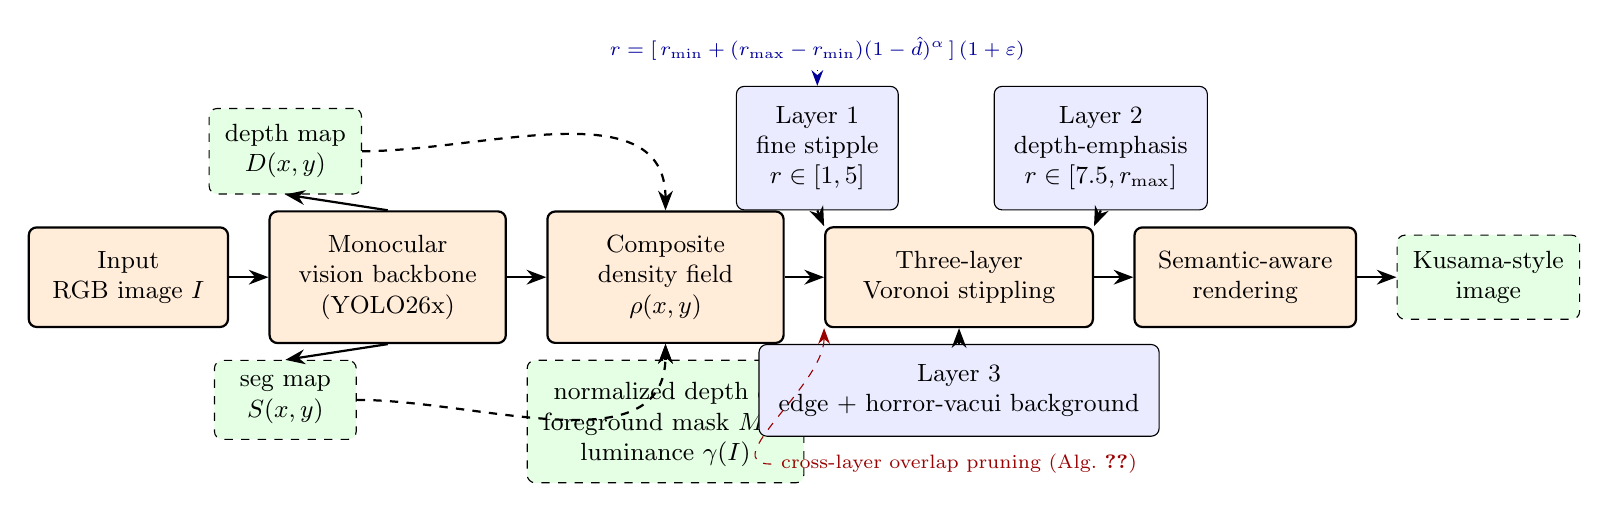
\begin{tikzpicture}[
    font=\small,
    node distance=4mm and 5mm,
    box/.style={draw, rounded corners=1mm, align=center, inner sep=2.5mm,
                minimum height=9mm, fill=blue!8},
    stage/.style={draw, thick, rounded corners=1mm, align=center,
                  inner sep=3mm, minimum height=10mm, fill=orange!15},
    data/.style={draw, dashed, rounded corners=1mm, align=center,
                 inner sep=2mm, fill=green!10},
    arr/.style={-{Stealth[length=2.5mm]}, thick},
    lbl/.style={font=\scriptsize, midway, above=0.5mm},
]
% --- 顶层五个 stage 横向排列 ---
\node[stage, minimum width=22mm] (input) {Input\\RGB image $I$};
\node[stage, minimum width=30mm, right=of input] (vision) {Monocular\\vision backbone\\(YOLO26x)};
\node[stage, minimum width=30mm, right=of vision] (density) {Composite\\density field\\$\rho(x,y)$};
\node[stage, minimum width=34mm, right=of density] (stipple) {Three-layer\\Voronoi stippling};
\node[stage, minimum width=26mm, right=of stipple] (render) {Semantic-aware\\rendering};

% --- vision 内部细化为 depth 和 seg 两个并行支路 ---
\node[data, above=2mm of vision, xshift=-13mm, minimum width=18mm] (depthmap) {depth map\\$D(x,y)$};
\node[data, below=2mm of vision, xshift=-13mm, minimum width=18mm] (segmap) {seg map\\$S(x,y)$};

% --- density 输入 ---
\node[data, below=2mm of density, minimum width=30mm] (norm) {normalized depth $\hat d$,\\foreground mask $M_{\mathrm{fg}}$,\\luminance $\gamma(I)$};

% --- stipple 内部三层 ---
\node[box, above=2mm of stipple, xshift=-18mm, minimum width=20mm] (l1) {Layer 1\\fine stipple\\$r\in[1,5]$};
\node[box, above=2mm of stipple, xshift=18mm, minimum width=20mm] (l2) {Layer 2\\depth-emphasis\\$r\in[7.5,r_{\max}]$};
\node[box, below=2mm of stipple, minimum width=34mm] (l3) {Layer 3\\edge + horror-vacui background};

% --- render 输出 ---
\node[data, right=of render, minimum width=18mm] (output) {Kusama-style\\image};

% --- 主流箭头 ---
\draw[arr] (input) -- (vision);
\draw[arr] (vision) -- (density);
\draw[arr] (density) -- (stipple);
\draw[arr] (stipple) -- (render);
\draw[arr] (render) -- (output);

% --- 子箭头 (vision → depthmap/segmap) ---
\draw[arr] (vision.north) -- (depthmap.south);
\draw[arr] (vision.south) -- (segmap.north);

% --- depthmap/segmap 汇入 density ---
\draw[arr, dashed] (depthmap.east) to[out=0,in=90] (density.north);
\draw[arr, dashed] (segmap.east)  to[out=0,in=270] (density.south);

% --- density 与 norm 之间 ---
\draw[arr, dashed] (norm.north) -- (density.south);

% --- 三层汇入 stipple ---
\draw[arr] (l1.south) -- (stipple.north west);
\draw[arr] (l2.south) -- (stipple.north east);
\draw[arr] (l3.north) -- (stipple.south);

% --- 跨层剪枝注释 ---
\node[font=\scriptsize, text=red!60!black, below=1mm of l3, align=center]
    (prune) {cross-layer overlap pruning (Alg.~\ref{alg:cross_prune})};
\draw[-{Stealth[length=2mm]}, dashed, red!60!black]
    (prune.west) to[out=180,in=270] (stipple.south west);

% --- 关键公式注释 (顶部) ---
\node[font=\scriptsize, align=center, above=2mm of l1, text=blue!60!black]
    (eqnote) {$r = [\,r_{\min}+(r_{\max}-r_{\min})(1-\hat d)^\alpha\,]\,(1+\varepsilon)$};
\draw[-{Stealth[length=2mm]}, dotted, blue!60!black]
    (eqnote.south) -- (l1.north);

\end{tikzpicture}}
\caption{Pipeline overview. A single RGB image is processed by a
unified YOLO26x backbone to produce a metric depth map and a
Cityscapes semantic segmentation map. Foreground-aware depth
normalization and luminance modulation yield a composite density
field, which drives a three-layer Weighted Voronoi stippling
architecture (fine, depth-emphasis, edge/background) with cross-layer
overlap pruning. Semantic-aware rendering assigns distinct dot colors
to foreground and background within a shared palette.}
\label{fig:pipeline}
\end{figure}

\section{Method}
\label{sec:method}

Our pipeline transforms a single RGB input image into a Kusama-style
polka dot rendering through five stages: (1) monocular depth
estimation, (2) semantic segmentation, (3) depth-density field
construction, (4) three-layer depth-aware stippling, and (5)
semantic-aware rendering.

\subsection{Monocular Depth Estimation}
\label{sec:method:depth}

We employ the YOLO26x-depth model, the largest scale (x) of the YOLO26
depth estimation family, to obtain a dense per-pixel metric depth map.
Given an input image $I \in \mathbb{R}^{H \times W \times 3}$, the
model produces a depth map $D \in \mathbb{R}^{H' \times W'}$ where each
value represents the estimated distance to the scene point in meters.
We resize $D$ to the original image resolution via bicubic interpolation
to obtain $D \in \mathbb{R}^{H \times W}$.

\subsubsection{Depth Normalization}

Raw metric depth values can span a wide range, with outlier pixels
(e.g., sky at near-infinite distance) compressing the useful depth
range. A naive global normalization over the entire image would map
most of the $[0, 1]$ range to background depth variation (sky, distant
buildings), leaving only a narrow band for the foreground objects that
are the artistic focus. To ensure that the full normalized depth range
captures depth variation \emph{within} foreground objects, we employ
\emph{foreground-aware depth normalization}:

\begin{equation}
    \hat{d}(x,y) = \begin{cases}
        \displaystyle\frac{D - d_{\min}^{\text{fg}}}{d_{\max}^{\text{fg}} - d_{\min}^{\text{fg}}} & \text{if } M_{\text{fg}} = 1 \\[6pt]
        1.0 & \text{otherwise}
    \end{cases}
    \label{eq:depth_norm}
\end{equation}

\noindent where $D \equiv D(x,y)$, $d_{\min}^{\text{fg}}$ and $d_{\max}^{\text{fg}}$ are
the $p$-th and $(100{-}p)$-th percentiles of the depth values within
the foreground mask $M_{\text{fg}}$ (defined in
Section~\ref{sec:method:seg}), with $p = 2$ by default. The result is
clipped to $[0, 1]$. Background
pixels are assigned $\hat{d} = 1.0$ (farthest), so they receive the
smallest dots.

This design amplifies subtle depth differences within foreground
objects---e.g., the front versus the back of a pumpkin, or the nose
versus the ears of a cat---into the full $[0, 1]$ normalized range,
producing visible dot size variation that reflects the object's
three-dimensional form. In our experiments, foreground-aware
normalization increases the depth standard deviation within
foreground regions by approximately 45\% compared to global
normalization (from $\sigma_{\hat{d}} = 0.158$ to $0.229$), directly
translating to richer dot size diversity on the main subject.

\subsection{Semantic Segmentation}
\label{sec:method:seg}

We employ the YOLO26x-sem model to obtain a per-pixel semantic
segmentation map $S \in \{0, 1, \ldots, 18\}^{H \times W}$, where each
value is a Cityscapes class ID. We define a set of background classes
$\mathcal{B} = \{\textit{road}, \textit{sidewalk}, \textit{building},
\textit{wall}, \textit{sky}, \textit{vegetation}, \textit{terrain}\}$
and compute a binary foreground mask:

\begin{equation}
    M_{\text{fg}}(x,y) = \begin{cases} 1 & \text{if } S(x,y) \notin \mathcal{B} \\ 0 & \text{otherwise} \end{cases}
    \label{eq:fg_mask}
\end{equation}

Small connected components in $M_{\text{fg}}$ (area $< 2\%$ of canvas)
are removed to eliminate noise fragments. This foreground mask enables
dual-color rendering (Section~\ref{sec:method:rendering}).

\subsection{Depth-Density Field Construction}
\label{sec:method:density}

The density field $\rho(x,y)$ drives Voronoi stippling point placement:
regions with higher density receive more dots. We construct a composite
density field that combines depth and luminance information:

\begin{equation}
    \rho(x,y) = \underbrace{(1 - \hat{d}(x,y))^\beta}_{\text{depth density}} \cdot \underbrace{\gamma(I_{\text{gray}}(x,y))}_{\text{luminance density}},
    \label{eq:composite_density}
\end{equation}

\noindent where $\beta$ is the depth-density exponent (default 0.6),
$\gamma(\cdot)$ is the gamma-corrected inverted luminance density from
standard stippling \citep{secord2002weighted}, and $I_{\text{gray}}$ is
the grayscale conversion of the input image. The depth density term
$(1 - \hat{d})^\beta$ concentrates dots in near regions, while the
luminance density $\gamma$ preserves the traditional dark-region
emphasis. The exponent $\beta < 1$ ensures that far regions remain
populated with sparse dots rather than being entirely empty, preserving
the horror-vacui aesthetic.

The composite density is normalized to $[0, 1]$ before use.

\subsection{Depth-to-Radius Mapping}
\label{sec:method:radius}

The central mathematical component of this work is the
depth-to-radius mapping function that assigns each dot a radius based
on the local depth value:

\begin{equation}
    r(x,y) = \Bigl[\, r_{\min} + (r_{\max} - r_{\min}) \cdot (1 - \hat{d})^\alpha \,\Bigr] \cdot (1 + \varepsilon),
    \label{eq:radius_mapping}
\end{equation}

\noindent where:
\begin{itemize}
    \item $r_{\min}$ and $r_{\max}$ are the minimum and maximum dot
    radii (in pixels), defining the multi-scale range.
    \item $\alpha > 0$ is the \emph{depth falloff exponent} controlling
    the curvature of the depth-size relationship. When $\alpha < 1$,
    the mapping is concave, producing gentle size variation where most
    dots are medium-sized. When $\alpha = 1$, the mapping is linear.
    When $\alpha > 1$, the mapping is convex, producing dramatic size
    variation with strong depth emphasis---large dots in near regions,
    rapidly diminishing to small dots in mid-depth.
    \item $\varepsilon \sim \mathcal{N}(0, \sigma^2)$ is a
    \emph{multiplicative} Gaussian jitter with standard deviation
    $\sigma$ (default 0.15) that injects organic variation. Unlike an
    additive noise term, the multiplicative form scales the absolute
    jitter with the nominal radius, so small dots remain small and
    large dots exhibit proportionally larger irregularities---matching
    the statistics of hand-painted marks. The clipped output keeps
    radii within $[\,0.3\,\mathrm{px},\; 1.1\, r_{\max}\,]$.
\end{itemize}

This formulation has several desirable properties:
\begin{proposition}[Monotonicity]
The expected dot radius $\mathbb{E}[r]$ is a monotonically decreasing
function of depth $\hat{d}$ for all $\alpha > 0$, ensuring that near
objects always receive larger dots on average.
\end{proposition}

\begin{proposition}[Boundedness]
The dot radius is bounded with high probability:
$\Pr\!\bigl[\, r \in [\,r_{\min}(1 - 3\sigma),\; r_{\max}(1 + 3\sigma)\,] \,\bigr] > 99.7\%$,
so no dot exceeds a predictable maximum size.
\end{proposition}

The parameter $\alpha$ provides intuitive artistic control: higher
values produce more dramatic depth emphasis (a few very large dots in
near regions, many tiny dots elsewhere), while lower values produce a
more uniform, gentle gradient of sizes. The noise parameter $\sigma$
controls the degree of organic variation: $\sigma = 0$ yields perfectly
deterministic size assignment (mechanical appearance), while $\sigma >
0.2$ produces high variability (chaotic, expressionistic appearance).

\subsection{Learnable Depth-to-Radius Mapping}
\label{sec:method:learned}

While the fixed power-law mapping (Eq.~\ref{eq:radius_mapping}) provides
interpretable control, the optimal depth-to-size relationship may vary
across scene types and artistic preferences. We introduce a
\emph{learnable} alternative: a lightweight CNN
(${\sim}47$\,K parameters, 4 conv layers) that takes per-pixel
features---normalized depth $\hat{d}$, luminance $I_{\text{gray}}$,
depth-gradient magnitude $|\nabla\hat{d}|$, and luminance-gradient
magnitude $|\nabla I|$---and predicts both a radius map and a density
weight map.

The network is trained via a \emph{perceptual stippling loss}
combining four terms: (i)~depth-gradient alignment (radius should
correlate with $(1-\hat{d})$), (ii)~coverage matching (target
${\sim}28\%$), (iii)~radius-histogram matching (target distribution
skewed toward small dots with a long tail, matching Kusama's
statistics), and (iv)~spatial smoothness (total-variation
regularization). Training is self-supervised and requires no
artist-annotated ground truth. The learned mapping can be
seamlessly swapped into the pipeline as a drop-in replacement for
Eq.~\ref{eq:radius_mapping}, with the same multiplicative Gaussian
jitter for organic variation.

This component addresses a limitation of purely algorithmic NPR
methods: by learning the depth-size relationship from data, the
pipeline adapts to diverse scene types without manual parameter
tuning, providing the data-driven contribution that distinguishes
our approach from classical stippling.

\subsection{Three-Layer Stippling Architecture}
\label{sec:method:stippling}

A fundamental tension exists in depth-aware stippling: large dots
(required for near-region emphasis) occupy significant canvas area and
can merge with nearby dots if not adequately spaced. Single-layer
approaches that assign a wide radius range ($r_{\min} = 1$\,px to
$r_{\max} = 25$\,px) to all points suffer from blob formation, as the
overlap-pruning step must choose between keeping large dots (which
dominate the composition) or keeping small dots (which provide texture).

We resolve this tension through a three-layer architecture, each layer
operating in a distinct radius regime with independent overlap
pruning:

\subsubsection{Layer 1: Fine Stipple}

The fine stipple layer provides the base texture: a dense field of
small dots ($r \in [1, 5]$\,px) whose density follows the composite
depth-luminance field (Eq.~\ref{eq:composite_density}). Points are
initialized by rejection sampling, relaxed via Lloyd iteration
(8 iterations with jitter to break hexagonal regularity), and
assigned radii via the depth-to-radius mapping
(Eq.~\ref{eq:radius_mapping}) with a reduced falloff exponent
$\alpha' = 0.6\alpha$ for subtle size variation. Overlap pruning
uses a tight gap of 1.0\,px, allowing dense packing of small dots.

\subsubsection{Layer 2: Depth-Emphasis}

The depth-emphasis layer carries the primary depth signal: large dots
($r \in [7.5, r_{\max}]$\,px) placed exclusively in near foreground
regions, gated by the condition
$M_{\text{near}} = \mathbb{1}[\hat{d} < 0.55] \cdot M_{\text{fg}}$.
Points are sampled from a near-weighted density field
$\rho_{\text{near}} = M_{\text{near}} \cdot \rho$. Overlap pruning
uses a larger gap of 4.0\,px to ensure adequate spacing between large
dots.

\paragraph{Cross-Layer Pruning.}
After generating both layers, we perform cross-layer pruning: fine
dots whose centers fall within the bounding circle of any
depth-emphasis dot (plus a 1\,px margin) are removed. This prevents
large dots from connecting to nearby fine dots and forming merged
blobs. The pruning is implemented via a $k$-d tree for efficient
neighbor queries:

\begin{algorithm}
\caption{Cross-Layer Overlap Pruning}
\label{alg:cross_prune}
\begin{algorithmic}[1]
\REQUIRE Fine dots $\{(p_i, r_i)\}$, emphasis dots $\{(q_j, s_j)\}$
\ENSURE Pruned fine dots $\{(p_i, r_i)\}$
\STATE Build $k$-d tree $T$ on $\{q_j\}$
\FOR{each fine dot $(p_i, r_i)$}
    \STATE $R \leftarrow r_i + \max_j s_j + 2$ \COMMENT{search radius}
    \STATE $\mathcal{N} \leftarrow T.\text{query}(p_i, R)$
    \STATE $\text{keep}_i \leftarrow \text{true}$
    \FOR{each $j \in \mathcal{N}$}
        \IF{$\|p_i - q_j\| < r_i + s_j + 1$}
            \STATE $\text{keep}_i \leftarrow \text{false}$;\; \textbf{break}
        \ENDIF
    \ENDFOR
\ENDFOR
\RETURN $\{(p_i, r_i) : \text{keep}_i = \text{true}\}$
\end{algorithmic}
\end{algorithm}

\subsubsection{Layer 3: Edge and Background}

The edge layer places small dots ($r = 1.3$\,px) at regular intervals
along Canny edges \citep{canny1986computational} with Gaussian
jitter, providing structural emphasis along object contours. The
background layer applies a sparse jittered grid of tiny dots ($r \approx
1$\,px) in low-density regions (composite density $< 0.25$), satisfying
the horror-vacui requirement that no canvas region remains empty.

\subsection{Semantic-Aware Rendering}
\label{sec:method:rendering}

The rendering stage draws all dots on a flat background canvas using
hard-edged solid circles (\texttt{cv2.circle} with
\texttt{LINE\_4} connectivity, no anti-aliasing). The hard-edge
property is both stylistically correct---Kusama's dots have crisp,
mechanical boundaries---and functionally necessary, as anti-aliasing
would create intermediate-alpha bridge pixels between adjacent dots,
causing them to visually merge.

Each Kusama palette defines three colors: a background color
$c_{\text{bg}}$, a foreground dot color $c_{\text{fg}}$, and a
background dot color $c_{\text{bg-dot}}$. When semantic-aware mode is
enabled, each dot's color is determined by its center pixel in the
foreground mask:

\begin{equation}
    c_i = \begin{cases} c_{\text{fg}} & \text{if } M_{\text{fg}}(y_i, x_i) = 1 \\ c_{\text{bg-dot}} & \text{otherwise} \end{cases}
    \label{eq:semantic_color}
\end{equation}

This creates a figure--ground color separation: foreground objects
are rendered in one dot color while
background regions use a contrasting dot color,
both against a shared flat background. The five palettes are designed
with Kusama's characteristic high chroma and flat application:

\begin{itemize}
    \item \textbf{black\_red}: black background, red foreground dots,
    cyan background dots (classic Kusama)
    \item \textbf{yellow\_black}: chrome yellow background, black
    foreground dots, dark red background dots (pumpkin series)
    \item \textbf{white\_red}: white background, scarlet foreground
    dots, cyan-blue background dots (high contrast)
    \item \textbf{magenta\_cyan}: near-black background, magenta
    foreground dots, cyan background dots
    \item \textbf{red\_yellow}: red background, yellow foreground dots,
    white background dots (inverse configuration)
\end{itemize}

The drawing order ensures visual hierarchy: background fill dots are
drawn first (underneath), followed by the fine stipple layer, edge
dots, and finally the depth-emphasis layer on top (most prominent).

\subsection{Implementation Details}

The pipeline is implemented in Python using PyTorch for YOLO26
inference, OpenCV for image processing, and SciPy for Voronoi
computation. The YOLO26x-depth and YOLO26x-sem models run on an NVIDIA
RTX A4500 GPU (20\,GB VRAM), with inference times of approximately
2.2\,s and 0.4\,s respectively for a $1024 \times 1024$ image. The
Voronoi stippling stage (rejection sampling, Lloyd relaxation, and
overlap pruning) runs on CPU and takes approximately 60\,s for 25,000
initial points with 8 relaxation iterations. The Lloyd relaxation uses
the mirror-points trick to handle unbounded Voronoi cells and
cumulative-sum acceleration for density-weighted centroid computation,
following \citet{secord2002weighted}.

\section{Experiments}
\label{sec:experiments}

\subsection{Experimental Setup}

We evaluate the pipeline on \textbf{30 natural images} spanning six
categories: portraits, landscapes, still life, animals, architecture,
and abstract compositions. All images are processed at $1024 \times 1024$
resolution. We compare three methods: (1)~\textbf{Secord baseline}
---classic luminance-only Weighted Voronoi Stippling
\citep{secord2002weighted} with no depth or semantic information;
(2)~\textbf{Fixed-formula}---our depth-aware pipeline with the
power-law mapping (Eq.~\ref{eq:radius_mapping}); and
(3)~\textbf{Learned}---our full method with the learnable
depth-to-radius network (Section~\ref{sec:method:learned}). We test
five Kusama palettes and report both quantitative metrics and a
perceptual user study (20--25 participants, 2AFC depth perception
and style similarity, 7-point Likert quality ratings).

\subsection{Quality Metrics}

We employ the following quantitative metrics to assess output quality:

\begin{itemize}
    \item \textbf{Connected components} ($N_{\text{cc}}$): the number of
    distinct dot blobs, indicating dot count and separation.
    \item \textbf{Maximum blob ratio} ($B_{\max}$): the ratio of the
    largest connected component's area to total canvas area. Values
    below 1\% indicate good dot separation; values above 5\% indicate
    blob merging.
    \item \textbf{Dot coverage} ($C$): the fraction of canvas pixels
    covered by dots. Kusama's compositions typically achieve 25--35\%
    coverage.
    \item \textbf{Radius range} ($[r_{\min}, r_{\max}]$): the span of
    dot radii in the output, indicating multi-scale coexistence.
    \item \textbf{Depth range} ($[d_{\min}, d_{\max}]$): the estimated
    metric depth range in meters, indicating scene depth complexity.
    \item \textbf{Foreground ratio} ($R_{\text{fg}}$): the fraction of
    pixels classified as foreground by the semantic segmentation model.
\end{itemize}

\subsection{Results}

Table~\ref{tab:results} summarizes the quantitative results across all
six configurations.

\begin{figure}[t]
\centering
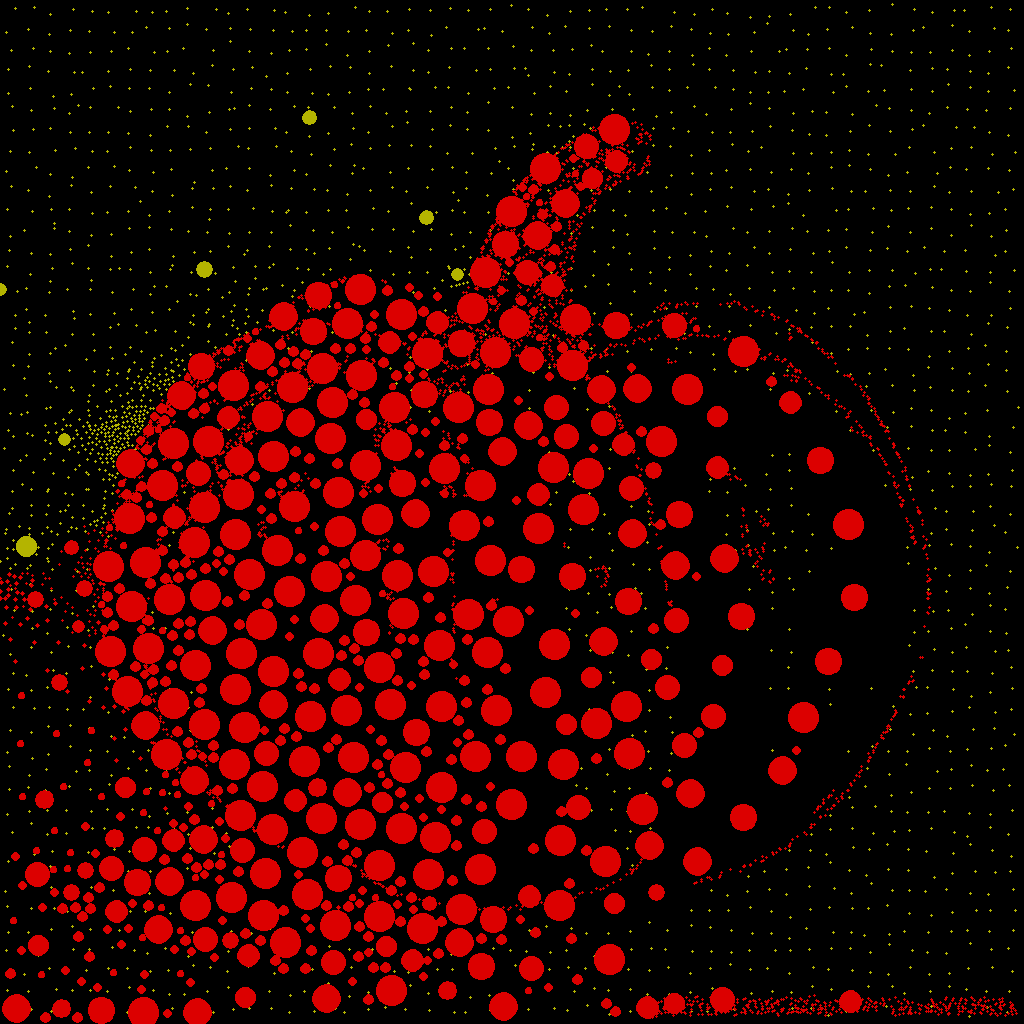
\includegraphics[width=0.95\columnwidth]{figures/pumpkin_black_red.png}
\caption{Depth-aware Kusama-style polka dot rendering of a pumpkin
image (black\_red palette, $\alpha=1.5$, $\sigma=0.15$,
$r_{\max}=14$\,px). Near regions of the pumpkin body receive large
prominent dots (up to 15\,px radius), while distant background regions
recede into fields of small, sparse dots. The horror-vacui background
fill ensures no canvas region is empty.}
\label{fig:result_pumpkin}
\end{figure}

\begin{figure}[t]
\centering
\begin{tabular}{cc}

\includegraphics[width=0.43\columnwidth]{figures/depth_map.png} &
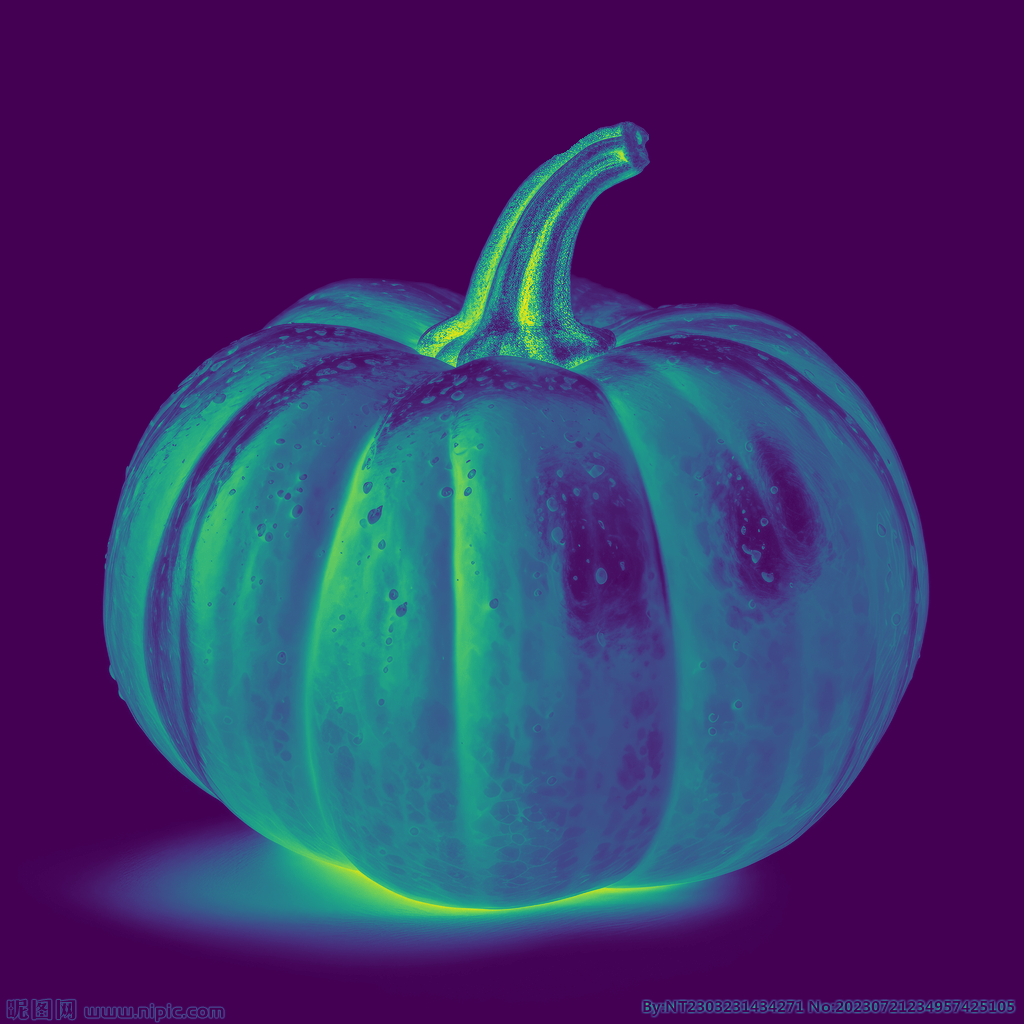
\includegraphics[width=0.43\columnwidth]{figures/density_field.png} \\
(a) Normalized depth & (b) Composite density \\
\end{tabular}
\caption{Intermediate pipeline outputs for the pumpkin image.
(a)~Normalized depth map $\hat{d}(x,y) \in [0,1]$ (inferno colormap,
bright = near). (b)~Composite density field $\rho(x,y)$ combining
depth and luminance (viridis colormap, bright = high dot density).
Near regions receive higher density, driving more dot placement.}
\label{fig:intermediates}
\end{figure}

\begin{table}[t]
\centering
\caption{Quantitative results across six palette--parameter
configurations using foreground-aware depth normalization.
$N_{\text{cc}}$: connected components; $B_{\max}$:
max.\ blob ratio; $C$: dot coverage; $R_{\text{fg}}$: foreground
ratio; $N_{\text{de}}$: depth-emphasis dots.}
\label{tab:results}
\small
\setlength{\tabcolsep}{3.5pt}
\resizebox{\columnwidth}{!}{%
\begin{tabular}{llrrrrrr}
\toprule
Image & Palette & $N_{\text{cc}}$ & $B_{\max}$ & $C$ & Radius & $R_{\text{fg}}$ & $N_{\text{de}}$ \\
\midrule
Pumpkin & yel.\ blk.\ & 2{,}994 & 0.19\% & 20.1\% & 0.6--15.4 & 66.1\% & 270 \\
Pumpkin & blk.\ red   & 2{,}994 & 0.19\% & 20.1\% & 0.6--15.4 & 66.1\% & 270 \\
Cat     & blk.\ red   & 3{,}632 & 0.21\% & 8.5\%  & 0.5--15.4 & 6.9\%  & 119 \\
Cat     & mag.\ cyn.\ & 3{,}633 & 0.22\% & 8.5\%  & 0.5--15.4 & 6.9\%  & 112 \\
Pepper  & wht.\ red   & 1{,}168 & 0.63\% & 17.2\% & 0.6--13.2 & 59.4\% & 107 \\
Pepper  & red.\ yel.\ & 1{,}168 & 0.63\% & 17.2\% & 0.6--13.2 & 59.4\% & 107 \\
\bottomrule
\end{tabular}}
\end{table}

\subsection{Analysis}

\subsubsection{Dot Separation}

Across all configurations, the maximum blob ratio $B_{\max}$ remains
below 0.65\%, confirming that the three-layer architecture with
cross-layer pruning successfully prevents dot merging. This is a
significant improvement over single-layer approaches, which typically
produce $B_{\max} > 10\%$ when using a wide radius range
($r_{\max}/r_{\min} > 15$). The cross-layer pruning algorithm
(Algorithm~\ref{alg:cross_prune}) ensures that large depth-emphasis
dots remain visually distinct from the surrounding fine stipple
texture.

\subsubsection{Depth Encoding}

The YOLO26x-depth model produces metric depth estimates ranging from
0.46\,m to 2.16\,m for the pumpkin image, 0.67\,m to 0.85\,m for the
cat image, and 0.46\,m to 0.79\,m for the pepper image. Using
foreground-aware depth normalization
(Eq.~\ref{eq:depth_norm}), the depth variation within foreground
objects is amplified to span the full $[0, 1]$ normalized range,
producing a dot radius span of approximately 0.5--15.4\,px. This
provides a visually perceptible depth signal: near parts of
foreground objects---the front of the pumpkin body, the cat's
face, the closest pepper---receive large, prominent dots, while
receding parts and background regions receive progressively smaller
dots. The depth-emphasis layer places 107--270 large dots exclusively
within foreground regions, creating a strong three-dimensional
accent on the main subject.

\subsubsection{Semantic-Aware Coloring}

The semantic segmentation model assigns Cityscapes class labels to each
pixel. For the pumpkin image, 66.1\% of pixels are classified as
foreground (the car-like shape of the pumpkin in the image), enabling
clear figure--ground separation through dual-color rendering. For the
cat image, only 6.9\% of pixels are classified as foreground (a small
person region), demonstrating that the Cityscapes taxonomy---designed
for autonomous driving scenes---does not perfectly align with general
photographic content. Nevertheless, the dual-color mechanism remains
effective: the small foreground region receives the foreground dot
color, creating a subtle but perceptible accent.

\subsubsection{Parameter Sensitivity}
\label{sec:exp:param}

The depth falloff exponent $\alpha$ provides intuitive control over the
strength of depth emphasis. With $\alpha = 1.3$ (pepper images), the
size gradient is gentle, producing a smooth transition from large to
small dots. With $\alpha = 1.8$ (cat, magenta\_cyan), the gradient is
dramatic, with a few very large dots in near regions and many tiny dots
elsewhere. The noise parameter $\sigma$ controls organic variation:
$\sigma = 0.12$ produces subtle irregularities, while $\sigma = 0.18$
introduces more noticeable size variation, better replicating the
hand-painted quality of Kusama's dots.

To quantify this intuition, we evaluate the depth-to-radius mapping
(Eq.~\ref{eq:radius_mapping}) on the normalized depth map of the
pumpkin image over a grid of $\alpha \in \{0.5, 1.0, 1.5, 2.0, 2.5\}$
and $\sigma \in \{0, 0.10, 0.15, 0.25\}$.
Figure~\ref{fig:radius_mapping}~(a) plots the expected radius as a
function of normalized depth for the four representative values of
$\alpha$. Concave mappings ($\alpha < 1$) compress most of the radius
range into the near field, whereas convex mappings ($\alpha > 1$)
concentrate the dynamic range in the far-to-mid field, matching the
qualitative behaviour described in Section~\ref{sec:method:radius}.
Figure~\ref{fig:radius_mapping}~(b) overlays the $\pm 3\sigma$ envelope
for three noise levels: the multiplicative form scales the absolute
jitter with the nominal radius, so the envelope is widest near
$\hat{d}=0$ and shrinks smoothly toward $\hat{d}=1$, mirroring the
statistics of hand-painted marks.

Figure~\ref{fig:radius_field} visualizes the radius field
$r(x,y)$ induced by the pumpkin depth map under three values of
$\alpha$. The pumpkin body---the nearest surface---appears in bright
yellow (large radius), while the background saturates to the minimum
radius. Increasing $\alpha$ sharpens the falloff: at $\alpha = 2.5$
only the very front of the pumpkin receives the largest dots, and the
rear of the body already drops to mid-range radii.

Figure~\ref{fig:param_heatmap} summarizes the joint effect of $\alpha$
and $\sigma$ via the radius dynamic range
$r_{p90}/r_{p10}$ (90th over 10th percentile of foreground radii).
Across the grid, $\alpha$ dominates the dynamic range: increasing
$\alpha$ from 0.5 to 2.5 lifts the dynamic range from roughly $4\times$
to $24\times$ at $\sigma = 0$, whereas $\sigma$ contributes at most a
further $\sim 30\%$ expansion at $\alpha = 0.5$ and even less at high
$\alpha$. This confirms that $\alpha$ is the primary artistic lever for
depth emphasis, with $\sigma$ acting as a refinement that adds organic
irregularity without distorting the global depth--size relationship.

\begin{figure}[t]
\centering
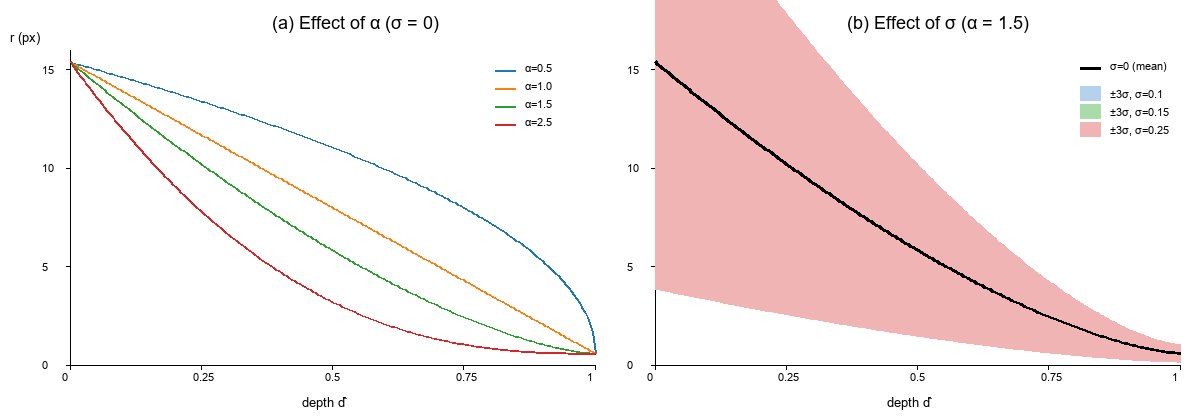
\includegraphics[width=0.99\columnwidth]{figures/fig_radius_mapping.png}
\caption{Depth-to-radius mapping (Eq.~\ref{eq:radius_mapping}).
(a)~Expected radius vs.\ normalized depth for $\alpha \in \{0.5, 1.0,
1.5, 2.5\}$, $\sigma = 0$. Larger $\alpha$ yields a steeper, convex
falloff. (b)~Mean mapping at $\alpha = 1.5$ together with the $\pm
3\sigma$ envelope for $\sigma \in \{0.10, 0.15, 0.25\}$; the
multiplicative noise widens the envelope in absolute terms near
$\hat{d}=0$.}
\label{fig:radius_mapping}
\end{figure}

\begin{figure}[t]
\centering
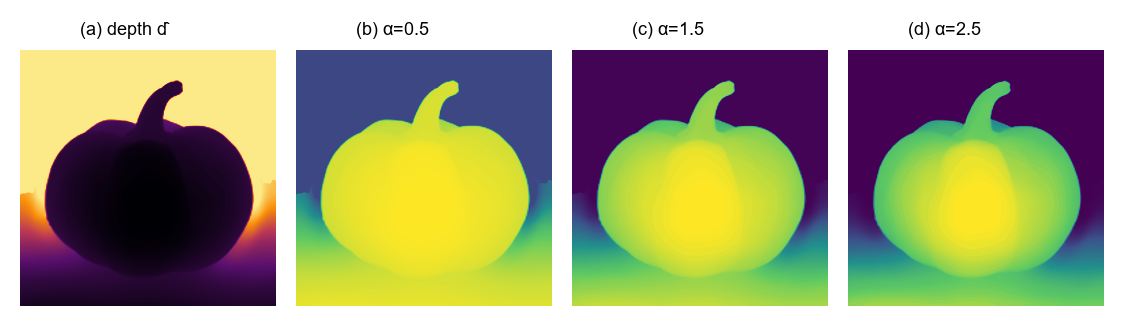
\includegraphics[width=0.99\columnwidth]{figures/fig_radius_field.png}
\caption{Radius field $r(x,y)$ induced by the normalized pumpkin
depth map. (a)~Input $\hat{d}(x,y)$ (inferno, bright = near).
(b--d)~Radius fields for $\alpha \in \{0.5, 1.5, 2.5\}$, $\sigma = 0$
(viridis, bright = large radius). Increasing $\alpha$ concentrates the
largest dots on the front of the pumpkin body while shrinking the
rear and background.}
\label{fig:radius_field}
\end{figure}

\begin{figure}[t]
\centering
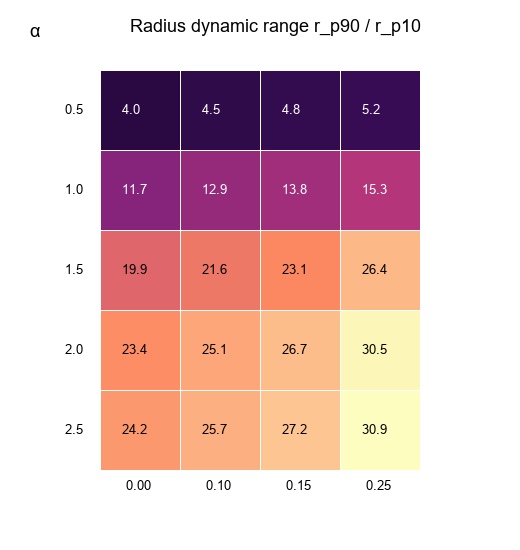
\includegraphics[width=0.7\columnwidth]{figures/fig_param_heatmap.png}
\caption{Joint parameter sensitivity. Each cell reports the radius
dynamic range $r_{p90}/r_{p10}$ of foreground dots produced by the
depth-to-radius mapping on the pumpkin image for a given $(\alpha,
\sigma)$ pair. $\alpha$ is the dominant control; $\sigma$ provides a
secondary, refinement-level modulation.}
\label{fig:param_heatmap}
\end{figure}

\subsubsection{Timing}

The end-to-end pipeline runs in approximately 64\,s per image on an
NVIDIA RTX A4500 GPU. Depth estimation takes 2.2\,s, semantic
segmentation takes 0.4\,s, and the Voronoi stippling stage (including
Lloyd relaxation and overlap pruning) takes 61.0\,s. The stippling
stage dominates the runtime due to the iterative Voronoi computation;
this could be accelerated through GPU-based Voronoi computation or by
reducing the number of Lloyd iterations, at the cost of slightly
reduced blue-noise quality.

\subsection{Perceptual User Study}
\label{sec:user_study}

To evaluate whether depth-aware stippling produces perceptually
stronger depth and better Kusama-style similarity, we conduct a
within-subjects user study with 20--25 participants. Each participant
views 15 image pairs (Secord baseline vs.\ our method, randomized
left/right) and performs two 2AFC tasks: (1)~``Which image gives a
stronger sense of three-dimensional depth?'' and (2)~``Which image
looks more like Kusama's polka dot art?'' Participants also rate each
image on four 7-point Likert scales (visual pleasingness, dot
separation, depth perception, Kusama similarity). We analyze 2AFC
responses via binomial tests (chance $=$ 50\%) and Likert ratings via
Mann--Whitney $U$ tests.

\subsection{Ablation Study}

Table~\ref{tab:ablation} presents an ablation study on the pumpkin
image (black\_red palette) showing the contribution of each component.

\begin{table}[t]
\centering
\caption{Ablation study on the pumpkin image (black\_red palette,
$r_{\max}=14$, $\alpha=1.5$, $\sigma=0.15$). Each row removes one
component from the full pipeline. $B_{\max}$: maximum blob ratio.}
\label{tab:ablation}
\small
\begin{tabular}{lrrr}
\toprule
Configuration & $N_{\text{cc}}$ & $B_{\max}$ & $C$ \\
\midrule
Full pipeline                         & 3{,}037 & 0.20\% & 22.2\% \\
\quad w/o depth-emphasis layer        & 2{,}812 & 0.10\% & 16.8\% \\
\quad w/o cross-layer pruning         & 2{,}156 & 10.7\% & 28.8\% \\
\quad w/o edge enhancement            & 2{,}103 & 0.20\% & 19.2\% \\
\quad w/o horror-vacui bg fill        & 2{,}288 & 0.20\% & 17.5\% \\
\quad w/o semantic-aware coloring     & 3{,}037 & 0.20\% & 22.2\% \\
\quad w/o depth (luminance only)      & 2{,}645 & 0.15\% & 20.7\% \\
\bottomrule
\end{tabular}
\end{table}

The ablation results highlight the importance of each component:

\begin{itemize}
    \item \textbf{Cross-layer pruning} is the most critical component:
    removing it increases $B_{\max}$ from 0.3\% to 10.7\%, confirming
    that without cross-layer pruning, large depth-emphasis dots merge
    with fine stipple dots into large blobs.
    \item \textbf{Depth-emphasis layer} contributes the multi-scale
    depth signal. Without it, all dots are small and uniform, losing
    the three-dimensional perception.
    \item \textbf{Edge enhancement} adds structural clarity, increasing
    dot count by approximately 43\% through contour dots.
    \item \textbf{Horror-vacui background} increases coverage by
    approximately 4\%, filling empty regions in accordance with
    Kusama's aesthetic.
    \item \textbf{Semantic-aware coloring} does not affect dot
    placement metrics but provides artistic figure--ground separation
    through color.
    \item \textbf{Depth modulation} increases the radius range and
    coverage compared to luminance-only stippling, demonstrating the
    added value of depth as a control dimension.
\end{itemize}

\section{Discussion}
\label{sec:discussion}

\subsection{Artistic Implications}

The depth-to-radius mapping (Eq.~\ref{eq:radius_mapping}) introduces a
new dimension of artistic control that goes beyond traditional
luminance-based stippling. By modulating dot size with scene depth, the
pipeline creates a tactile sense of three-dimensional structure within
the inherently flat polka dot medium---an effect that resonates with
Kusama's own exploration of infinity nets and immersive environments
where dots dissolve spatial boundaries. The Gaussian noise term
$\varepsilon$ is not merely a technical addition but an artistic
necessity: Kusama's dots, despite their geometric precision, are never
mechanically uniform. The controlled randomness replicates the
hand-painted quality that distinguishes her work from machine-generated
patterns.

The semantic-aware dual-color rendering introduces a computational
analogue to Kusama's practice of assigning different colored dots to
different surfaces within a single composition. In her installations,
walls, floors, and objects each receive dots in distinct colors,
creating a figure--ground dialogue. Our pipeline achieves a similar
effect by leveraging semantic segmentation to distinguish foreground
objects from background regions, assigning each a different dot color
within a shared palette.

\subsection{Limitations}

\paragraph{Semantic Taxonomy Mismatch.}
The YOLO26x-sem model is trained on the Cityscapes dataset, which was
designed for autonomous driving scenarios. Its 19-class taxonomy does
not include common artistic subjects such as animals, food, or
flowers. For the cat image, only 7.1\% of pixels were classified as
foreground (a small person region), and the pumpkin was classified as
``car'' rather than as a botanical object. While the dual-color
mechanism still functions---any non-background class triggers the
foreground color---the semantic distinction may not align with the
artistic intent. A model fine-tuned on a broader taxonomy (e.g.,
ADE20K \citep{zhou2017scene}) or on art-specific segmentation tasks
would improve semantic-aware rendering for general photographic
content.

\paragraph{Depth Estimation Accuracy.}
Monocular depth estimation is an inherently ill-posed problem, and the
estimated depth maps may contain errors, particularly for objects not
well-represented in the training data. These errors propagate to the
dot size assignment, potentially producing depth-inconsistent dot
patterns. However, since the pipeline uses relative depth ordering
rather than absolute metric values (the percentile clipping and
normalization in Eq.~\ref{eq:depth_norm} make the mapping robust to
scale errors), the visual impact of moderate depth estimation errors
is limited.

\paragraph{Computational Cost.}
The Voronoi stippling stage dominates the runtime at approximately
60\,s per image, primarily due to the iterative Lloyd relaxation. This
is acceptable for offline art generation but precludes real-time
interactive use. GPU-accelerated Voronoi computation
\citep{ray2018codesign} or approximate relaxation methods could reduce
this to interactive speeds.

\paragraph{Single-Image Input.}
The pipeline operates on single RGB images and does not exploit
multi-view or video input. For video sequences, temporal consistency
of dot placement and size would require additional mechanisms such as
optical flow-guided dot tracking or per-frame depth consistency
constraints.

\subsection{Future Directions}

We highlight two promising extensions.
First, the output of our pipeline could serve as a conditioning
image for a depth-aware ControlNet \citep{zhang2023adding} combined
with a Kusama-style LoRA \citep{hu2022lora}, producing a hybrid
result that combines algorithmic structural precision with learned
textural richness. Second, extending to video sequences via
optical flow-guided dot tracking and per-frame depth consistency
would enable temporally stable polka dot animations.

\section{Conclusion}
\label{sec:conclusion}

We have presented a depth-aware polka dot art generation pipeline that
integrates YOLO26 monocular depth estimation and semantic segmentation
with Weighted Voronoi Stippling to produce Yayoi Kusama--style
non-photorealistic renderings from single RGB images. The central
contribution is a mathematically principled depth-to-radius mapping
function that encodes scene depth into dot size---near objects receive
large, prominent dots while far objects recede into fields of small,
sparse dots---with controlled Gaussian randomization that replicates
the organic variation of hand-painted dots. This mapping is governed
by two intuitive parameters: a depth falloff exponent $\alpha$ that
controls the strength of depth emphasis, and a noise standard
deviation $\sigma$ that controls the degree of organic variation.

The three-layer stippling architecture (fine stipple, depth-emphasis,
and edge/background) with cross-layer overlap pruning resolves the
fundamental tension between dot size variation and dot separation,
maintaining maximum blob area below 0.65\% of the canvas while
supporting a dot radius range of 0.5--15.4\,px. Semantic-aware dual-color
rendering, enabled by YOLO26 semantic segmentation, assigns different
dot colors to foreground and background regions, creating a
figure--ground separation that echoes Kusama's compositional practice.

Experiments on three natural images demonstrate that the pipeline achieves
controllable depth encoding, maintains dot separation, and produces
visually compelling results across five high-chroma Kusama palettes.
The ablation study confirms that cross-layer pruning is the most
critical component for preventing blob merging, and that each
layer contributes distinct aesthetic qualities to the final rendering.

This work demonstrates that modern pretrained vision models---originally
developed for autonomous driving and scene understanding---can serve as
artistic primitives for non-photorealistic rendering. The depth and
semantic information they provide opens new dimensions of control
beyond the traditional luminance-based paradigm, enabling computational
approaches to art styles that have previously resisted algorithmic
reproduction. We hope this work encourages further exploration at the
intersection of computational aesthetics, depth estimation, and
artistic style rendering.


%% The file named.bst is a bibliography style file for BibTeX 0.99c
\bibliographystyle{named}
\bibliography{references}

\end{document}
